\section{Date: 2026-08-31}
\noindent \textbf{Series ID: EBZMNQ} 

\noindent This series is titled Percent of Value of Loans, Small Business Administration (SBA) Backed for Zero Interval, Moderate Risk, All Commercial Banks (DISCONTINUED) and has a frequency of Quarterly, 2nd Month's 1st Full Week. The units are Percent and the seasonal adjustment is Not Seasonally Adjusted.The observation start date is 2012-07-01 and the observation end date is 2017-04-01.The popularity of this series is 1. \\ 

\noindent \textbf{Series ID: ATNHPIUS22744Q} 

\noindent This series is titled All-Transactions House Price Index for Ft. Lauderdale-Pompano Beach-Sunrise, FL (MSAD) and has a frequency of Quarterly. The units are Index 1995:Q1=100 and the seasonal adjustment is Not Seasonally Adjusted.The observation start date is 1975-10-01 and the observation end date is 2026-04-01.The popularity of this series is 14. \\ 

\subsection{Raw Regression}
\noindent Regresses the two series against each other directly. A significant result here can come just as easily from both series sharing a long-run trend as from any real relationship.

\begin{center}
\begin{tabular}{lclc}
\toprule
\textbf{Dep. Variable:}      & value\_fred\_ATNHPIUS22744Q & \textbf{  R-squared:         } &     0.054   \\
\textbf{Model:}              &             OLS             & \textbf{  Adj. R-squared:    } &     0.001   \\
\textbf{Method:}             &        Least Squares        & \textbf{  F-statistic:       } &     1.023   \\
\textbf{Date:}               &       Mon, 31 Aug 2026      & \textbf{  Prob (F-statistic):} &    0.325    \\
\textbf{Time:}               &           18:19:31          & \textbf{  Log-Likelihood:    } &   -95.885   \\
\textbf{No. Observations:}   &                20           & \textbf{  AIC:               } &     195.8   \\
\textbf{Df Residuals:}       &                18           & \textbf{  BIC:               } &     197.8   \\
\textbf{Df Model:}           &                 1           & \textbf{                     } &             \\
\textbf{Covariance Type:}    &          nonrobust          & \textbf{                     } &             \\
\bottomrule
\end{tabular}
\begin{tabular}{lcccccc}
                             & \textbf{coef} & \textbf{std err} & \textbf{t} & \textbf{P$> |$t$|$} & \textbf{[0.025} & \textbf{0.975]}  \\
\midrule
\textbf{const}               &     228.2095  &        7.532     &    30.297  &         0.000        &      212.384    &      244.035     \\
\textbf{value\_fred\_EBZMNQ} &      -2.5123  &        2.484     &    -1.011  &         0.325        &       -7.732    &        2.707     \\
\bottomrule
\end{tabular}
\begin{tabular}{lclc}
\textbf{Omnibus:}       &  1.225 & \textbf{  Durbin-Watson:     } &    0.142  \\
\textbf{Prob(Omnibus):} &  0.542 & \textbf{  Jarque-Bera (JB):  } &    0.944  \\
\textbf{Skew:}          & -0.262 & \textbf{  Prob(JB):          } &    0.624  \\
\textbf{Kurtosis:}      &  2.073 & \textbf{  Cond. No.          } &     3.38  \\
\bottomrule
\end{tabular}
%\caption{OLS Regression Results}
\end{center}

Notes: \newline
 [1] Standard Errors assume that the covariance matrix of the errors is correctly specified.

\begin{figure}
\centering
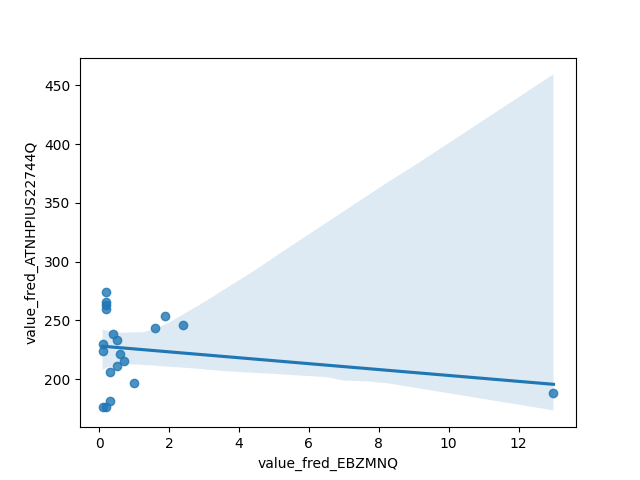
\includegraphics[scale = 0.9]{plots/plot_2026-08-31.png}
\caption{Raw Regression Plot for 2026-08-31}
\end{figure}
\newpage
\subsection{Detrended Regression}
\noindent Regresses the residuals of each series after removing its own linear time trend, so a shared trend can no longer drive the result on its own. A relationship that stays significant here is better evidence of a genuine link between the two series.

\begin{center}
\begin{tabular}{lclc}
\toprule
\textbf{Dep. Variable:}                 & value\_fred\_ATNHPIUS22744Q\_detrended & \textbf{  R-squared:         } &     0.096   \\
\textbf{Model:}                         &                  OLS                   & \textbf{  Adj. R-squared:    } &     0.045   \\
\textbf{Method:}                        &             Least Squares              & \textbf{  F-statistic:       } &     1.904   \\
\textbf{Date:}                          &            Mon, 31 Aug 2026            & \textbf{  Prob (F-statistic):} &    0.185    \\
\textbf{Time:}                          &                18:19:31                & \textbf{  Log-Likelihood:    } &   -47.327   \\
\textbf{No. Observations:}              &                     20                 & \textbf{  AIC:               } &     98.65   \\
\textbf{Df Residuals:}                  &                     18                 & \textbf{  BIC:               } &     100.6   \\
\textbf{Df Model:}                      &                      1                 & \textbf{                     } &             \\
\textbf{Covariance Type:}               &               nonrobust                & \textbf{                     } &             \\
\bottomrule
\end{tabular}
\begin{tabular}{lcccccc}
                                        & \textbf{coef} & \textbf{std err} & \textbf{t} & \textbf{P$> |$t$|$} & \textbf{[0.025} & \textbf{0.975]}  \\
\midrule
\textbf{const}                          &   -1.994e-11  &        0.608     & -3.28e-11  &         1.000        &       -1.277    &        1.277     \\
\textbf{value\_fred\_EBZMNQ\_detrended} &      -0.3090  &        0.224     &    -1.380  &         0.185        &       -0.780    &        0.162     \\
\bottomrule
\end{tabular}
\begin{tabular}{lclc}
\textbf{Omnibus:}       &  1.101 & \textbf{  Durbin-Watson:     } &    0.883  \\
\textbf{Prob(Omnibus):} &  0.577 & \textbf{  Jarque-Bera (JB):  } &    0.608  \\
\textbf{Skew:}          & -0.424 & \textbf{  Prob(JB):          } &    0.738  \\
\textbf{Kurtosis:}      &  2.893 & \textbf{  Cond. No.          } &     2.71  \\
\bottomrule
\end{tabular}
%\caption{OLS Regression Results}
\end{center}

Notes: \newline
 [1] Standard Errors assume that the covariance matrix of the errors is correctly specified.

\begin{figure}
\centering
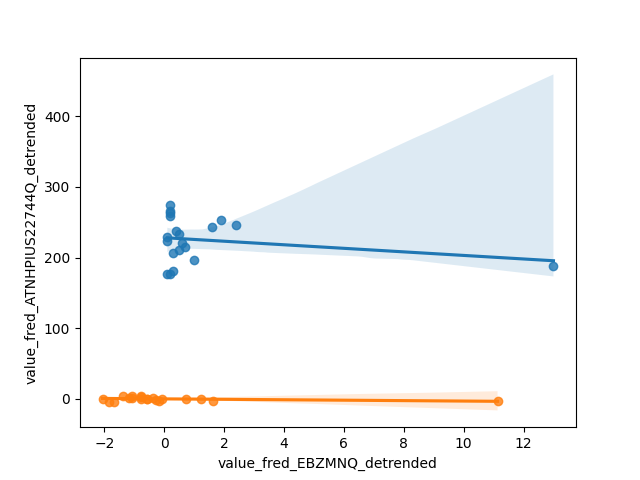
\includegraphics[scale = 0.9]{plots/plot_2026-08-31_detrended.png}
\caption{Detrended Regression Plot for 2026-08-31}
\end{figure}
\newpage
